\documentclass{article}

\usepackage{graphicx}
\usepackage{tikz}
\usepackage{tikzsymbols}
\usetikzlibrary{calc,patterns,shapes.geometric}
\pagestyle{empty}
\usepackage[margin=0pt]{geometry}
\geometry{papersize={14in,12in}}

\def\centerarc[#1](#2)(#3:#4:#5){\draw[#1] ($(#2)+({#5*cos(#3)},{#5*sin(#3)})$) arc (#3:#4:#5);}

\begin{document}
	\begin{figure}
		\centering
		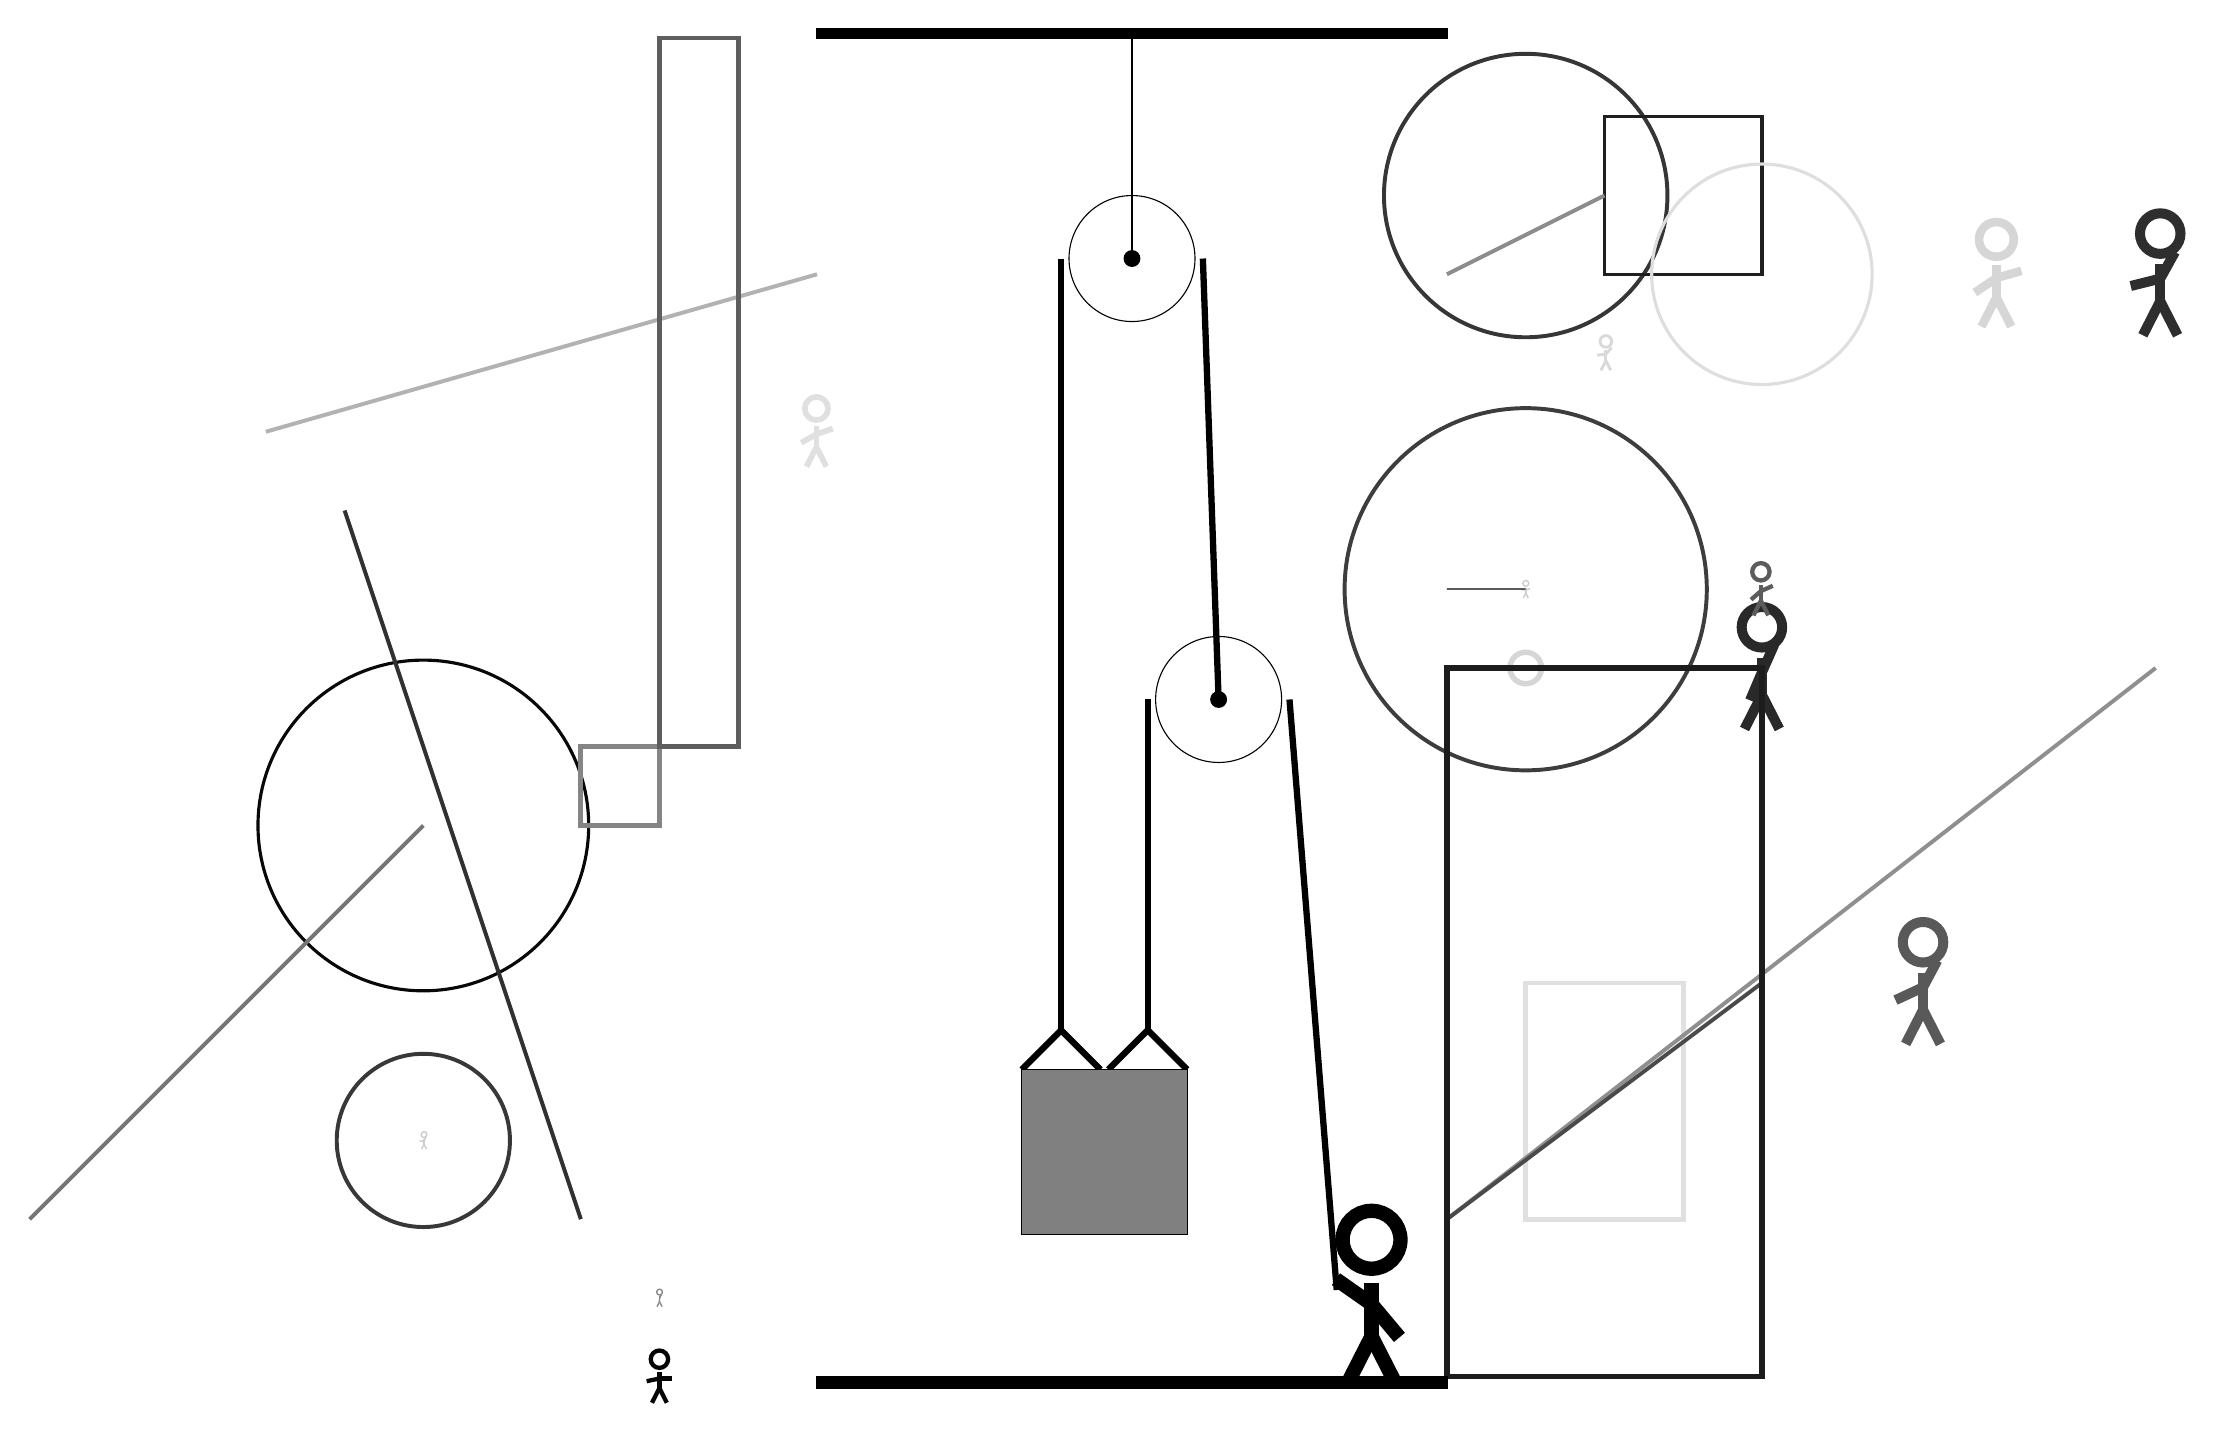
\begin{tikzpicture}
			%%%%% START %%%%%
			
			\draw[fill=black] (-2, 14) rectangle (6, 14.125);
			
			\draw (2, 11.2) circle (0.8);
			\draw[fill=black] (2, 11.2) circle (0.1);
			\draw[thick] (2, 11.2) -- (2, 14);
			
			\draw (3.1, 5.6) circle (0.8);
			\draw[fill=black] (3.1, 5.6) circle (0.1);
			
			\draw[line width = 0.8mm]  (0.6, 0.9) -- (1.1, 1.4) -- (1.6, 0.9);
			\draw[line width = 0.8mm]  (1.7, 0.9) -- (2.2, 1.4) -- (2.7, 0.9);
			\draw[fill=black!50] (0.6, 0.9) rectangle (2.7, -1.2);
			
			\draw[line width = 0.8mm] (1.1, 11.2) -- (1.1, 1.4);
			\centerarc[line width = 0.8mm](2, 11.2)(0:180:0.9);
			\draw[line width = 0.8mm] (2.9, 11.2) -- (3.1, 5.6);
			\draw[line width = 0.8mm] (2.2, 5.6) -- (2.2, 1.4);
			\centerarc[line width = 0.8mm](3.1, 5.6)(0:180:0.9);
			\draw[line width = 0.8mm] (4.0, 5.6) -- (4.6, -1.9);
			
			\node at (5, -2) {\Strichmaxerl[10][-35][-50]};
			
			\draw[line width=0.5mm, color=black!30](-2, 11) -- (-9, 9);
			
			\draw [line width=0.4mm, color=black!97](-7, 4) circle (2.1);
			\draw[line width=0.6mm, color=black!48] (-4, 4) rectangle (-5, 5);
			\node[line width=0.5mm, color=black!15] at (8, 10) {\Strichmaxerl[2][6][49]};
			\draw [line width=0.7mm, color=black!16](7, 6) circle (0.2);
			\node[line width=0.6mm, color=black!20] at (7, 7) {\Strichmaxerl[1][2][16]};
			\draw [line width=0.5mm, color=black!79](7, 12) circle (1.8);
			\node[line width=0.3mm, color=black!65] at (12, 2) {\Strichmaxerl[7][25][62]};
			\draw[line width=0.4mm, color=black!88] (8, 13) rectangle (10, 11);
			\node[line width=0.3mm, color=black!16] at (13, 11) {\Strichmaxerl[6][34][16]};
			\node[line width=0.3mm, color=black!82] at (15, 11) {\Strichmaxerl[7][14][61]};
			
			\draw[line width=0.6mm, color=black!12] (7, -1) rectangle (9, 2);
			\node[line width=0.4mm, color=black!45] at (-4, -2) {\Strichmaxerl[1][87][66]};
			\draw [line width=0.5mm, color=black!76](7, 7) circle (2.3);
			\draw[line width=0.5mm, color=black!44](6, -1) -- (15, 6);
			\draw[line width=0.5mm, color=black!71](10, 2) -- (6, -1);
			
			\node[line width=0.4mm, color=black!20] at (-7, 0) {\Strichmaxerl[1][1][67]};
			\node[line width=0.5mm, color=black!12] at (-2, 9) {\Strichmaxerl[4][29][19]};
			\draw[line width=0.5mm, color=black!81](-5, -1) -- (-8, 8);
			\node[line width=0.2mm, color=black!98] at (-4, -3) {\Strichmaxerl[3][12][0]};
			\node[line width=0.2mm, color=black!84] at (10, 6) {\Strichmaxerl[7][67][66]};
			
			\draw[line width=0.7mm, color=black!89] (6, 6) rectangle (10, -3);
			\draw[line width=0.5mm, color=black!54](-7, 4) -- (-12, -1);
			\draw [line width=0.6mm, color=black!47](12, 5) circle (0.0);
			\draw [line width=0.5mm, color=black!78](-7, 0) circle (1.1);
			
			\draw [line width=0.4mm, color=black!13](10, 11) circle (1.4);
			
			\node[line width=0.4mm, color=black!64] at (10, 7) {\Strichmaxerl[3][41][24]};
			\draw[line width=0.6mm, color=black!63] (-3, 14) rectangle (-4, 5);
			
			\draw[line width=0.3mm, color=black!64] (6, 7) rectangle (7, 7);
			\draw[line width=0.5mm, color=black!45](6, 11) -- (8, 12);
			
			\draw[fill=black] (-2, -3) rectangle (6, -3.15);
			
			%%%%% END %%%%%
		\end{tikzpicture}
	\end{figure}	
\end{document}